%%%%%%%%%%%%%%%%%%%%%%%%%%%%%%%%%%%%%%%%%%%%%%%%%%%%%%%%%%%%%%%%%%%%%%%%
%%
%% 序論.tex
%% LaTeX-2e 専用
%% 
%% 
%%        設計工学研究室 学位論文テンプレート
%%
%%                      作成日時    2010年 12月 17日
%%
%%%%%%%%%%%%%%%%%%%%%%%%%%%%%%%%%%%%%%%%%%%%%%%%%%%%%%%%%%%%%%%%%%%%%%%%

\chapter{序論}\label{chapter:序論}
第\ref{chapter:序論}章では,~を述べる.


\section{背景}

図の参照はFig. \ref{fig:sample}とする.

表の参照はTab. \ref{table:sample}とする.

参考文献の参照は\cite{実用的4足歩行機械}とする.

%図の挿入例
\begin{figure}[tbp]
  \begin{center}
    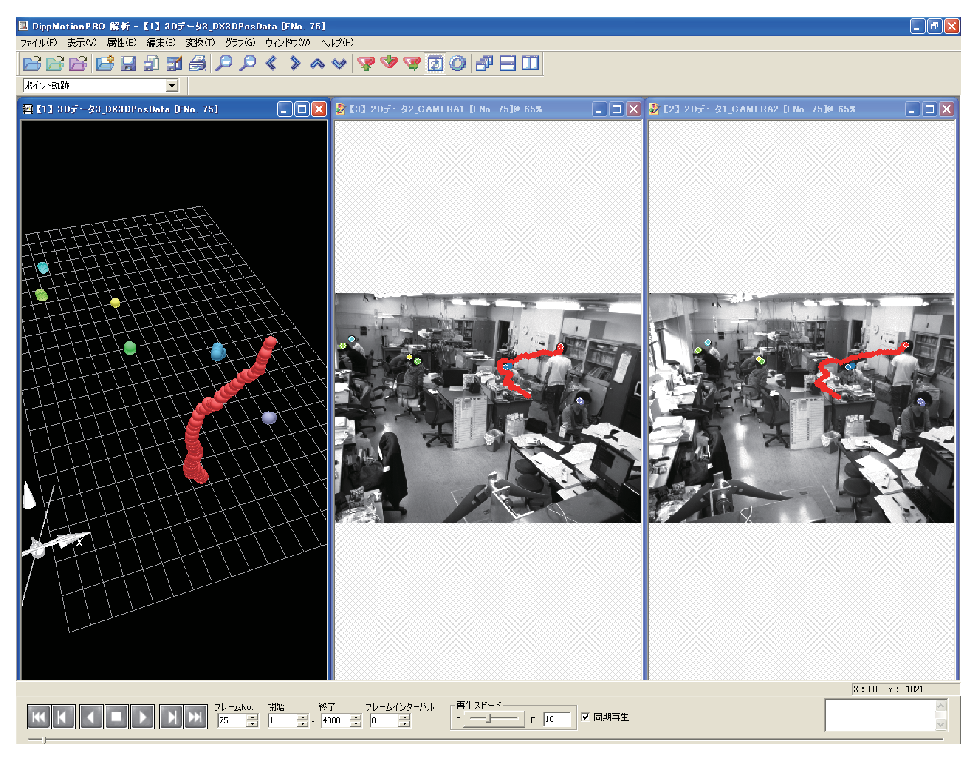
\includegraphics[width=50mm, clip]{figure1/sample.eps}
    \caption{Sample figure}
    \label{fig:sample}
  \end{center}
\end{figure}

%表の挿入例
\begin{table}[tbp]
    \caption{Sample table}
    \label{table:sample}
    \begin{center}
        \begin{tabular}{|c|c|c|}
        \hline
        Item & Spec. & Quantity  \\
        \hline\hline
        A & high & 10 \\
        \hline
        B & low & 100 \\
        \hline
        \end{tabular}
    \end{center}
\end{table}


\section{従来研究の技術動向}

\section{本論文の目的}

\section{本論文の構成}
本論文は,全x章から構成される.

第2章「理論と実施計画」では,~を述べる.hello
第3章「実験装置や開発機械」では,~を述べる.
第4章「実験」では,~を述べる.
第5章「結論」では本論文の結論と今後の課題を述べる.



